\documentclass{beamer}

%% Tema y configuraciones (misma anatomía de mis otros cursos)
\usetheme{Boadilla}
\usecolortheme{default}
\setbeamertemplate{navigation symbols}{}
\usepackage[utf8]{inputenc}
\usepackage[T1]{fontenc}
\usepackage{xcolor}
\usepackage{graphicx}
\usepackage{booktabs}
\usepackage{array}
\usepackage{colortbl}
\hypersetup{
    colorlinks=true,
    linkcolor=.,
    urlcolor=blue,
    citecolor=.,
}

%% Colores de apoyo (los mismos de la semana 5)
\definecolor{verdeok}{RGB}{39,124,74}
\definecolor{rojoal}{RGB}{198,40,40}
\definecolor{naranjal}{RGB}{230,126,34}
\definecolor{grisclaro}{RGB}{242,243,246}
\definecolor{azulcaso}{RGB}{28,60,120}

%% Encabezado
\title[06327-ECO]{Analítica para los negocios \\ 06327-ECO}
\subtitle{Semana 12: El gasto del próximo trimestre --- ¿se le puede ganar a la regla de Finanzas?}
\author{Eduard F. Martínez González, Ph.D.}
\institute[]{Departamento de Economía, Universidad Icesi}
\date{\textcolor{rojoal}{[fecha por definir]}}

%%=================================================
\begin{document}

\begin{frame}
\titlepage
\end{frame}

%%=================================================
\begin{frame}{Objetivo de la sesión}
\small
Hoy vuelve la pregunta de Finanzas: \textbf{cuánto gastará cada cliente el próximo trimestre}. Tres familias de modelos intentan ganarle a una regla de negocio de una línea.

\vspace{0.15cm}
\begin{itemize} \setlength{\itemsep}{0.16cm}
  \item La ruta lineal (Lasso), el árbol de regresión y el bosque, en el mismo sobre sellado.
  \item Cada ventaja, cliente a cliente y con su margen: ¿real o ruido?
  \item El diagnóstico: dónde se equivoca el mejor modelo.
  \item La decisión que junta las semanas 11 y 12: a quién llama Growth.
\end{itemize}

\vspace{0.15cm}
\begin{block}{La idea que gobierna la sesión}
Un torneo no siempre corona a un modelo: a veces corona un \textbf{hallazgo} --- dónde está la señal, dónde se acaba y dónde falla el pronóstico.
\end{block}
\end{frame}

%%=================================================
\begin{frame}{¿Dónde estamos en el curso?}
\small
\begin{itemize} \setlength{\itemsep}{0.22cm}
  \item \textbf{Semana 10:} la regla ``3 × gasto mensual'' le quitó la mitad al error de la media --- con márgenes que ni se tocan.
  \item \textbf{Semana 11:} el bosque empató con la regla del EDA en el cupo de Growth; lo que compró fue la perilla: un riesgo para cada cliente.
  \item \textbf{Semana 12 (hoy):} de categorías a números --- la misma maquinaria, ahora para predecir pesos.
\end{itemize}

\vspace{0.2cm}
\begin{block}{Lo que cambia hoy}
El error ya no es ``acertó o no'': se mide en \textbf{pesos}, y unos pocos clientes enormes pesan más que miles de pequeños.
\end{block}
\end{frame}

\begin{frame}[noframenumbering]{Roadmap}
\tableofcontents
\end{frame}

%%=================================================
\section{La pregunta y la vara}

\begin{frame}[noframenumbering]{Roadmap}
\tableofcontents[currentsection]
\end{frame}

\begin{frame}{La pregunta de hoy}
\small
\begin{block}{Frente de Finanzas}
``¿Cuánto gastará cada cliente de Cóndor el próximo trimestre?''
\end{block}

\vspace{0.15cm}
\centering
\footnotesize
\textbf{La tabla del líder que dejó la semana 10} (pesos por cliente, test de 1.600)
\vspace{0.05cm}

\begin{tabular}{lcr}
\toprule
Regla & MAE & RMSE \\
\midrule
Media de train & 328.494 ± 38.496 & 836.839 \\
\rowcolor{grisclaro} \textbf{3 × gasto mensual} & 168.728 ± 31.656 & 655.018 \\
\bottomrule
\end{tabular}

\raggedright
\small
\vspace{0.2cm}
Mismas 22 predictoras de la semana 11, con un cambio: ahora sale \texttt{abandono}, la variable del futuro para Finanzas (la fuga en espejo de la semana 10).
\end{frame}

\begin{frame}{Paso 1 · ¿Cómo se ve lo que queremos predecir?}
\small
\begin{center}
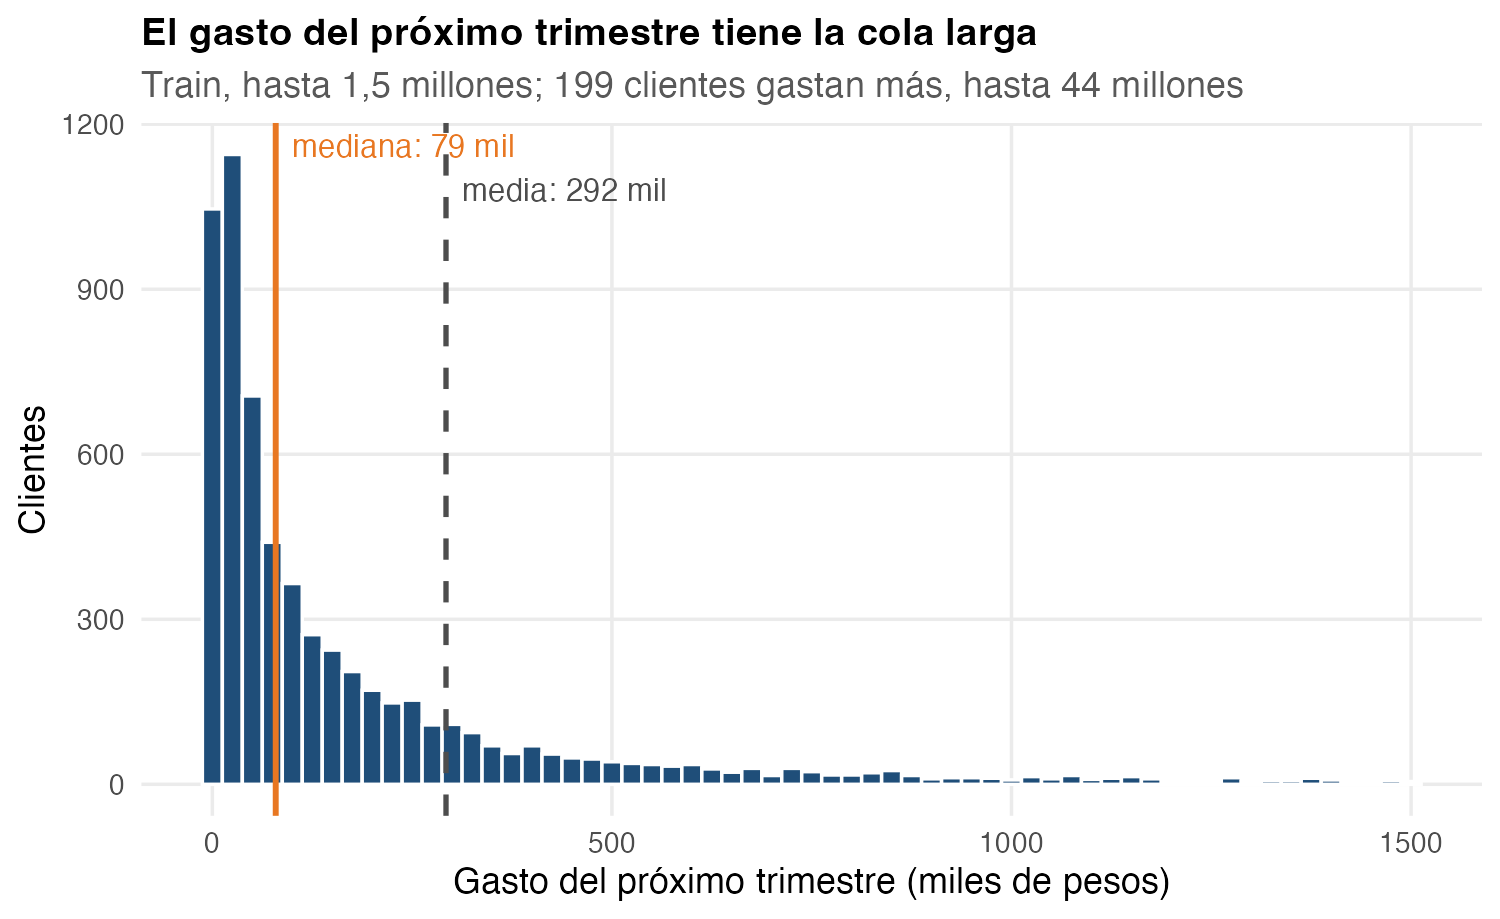
\includegraphics[width=0.6\textwidth]{pic/fig_s12_cola.png}
\end{center}
\vspace{-0.25cm}
\begin{itemize} \itemsep2pt
  \item Mediana \textbf{79.300}, media \textbf{292.378}, máximo \textbf{44.083.300} pesos: la media es casi cuatro veces la mediana.
\end{itemize}
\pause
\begin{alertblock}{Hallazgo 1}
\textbf{Cola larga}, como en la semana 6: unos pocos clientes pesan muchísimo en todo lo que se mide al cuadrado --- el RMSE y la forma como aprenden los tres modelos de hoy.
\end{alertblock}
\end{frame}

%%=================================================
\section{Tres familias de modelos}

\begin{frame}[noframenumbering]{Roadmap}
\tableofcontents[currentsection]
\end{frame}

\begin{frame}{Paso 2 · ¿Qué ecuación encuentra el Lasso?}
\small
\begin{columns}[T]
\column{0.58\textwidth}
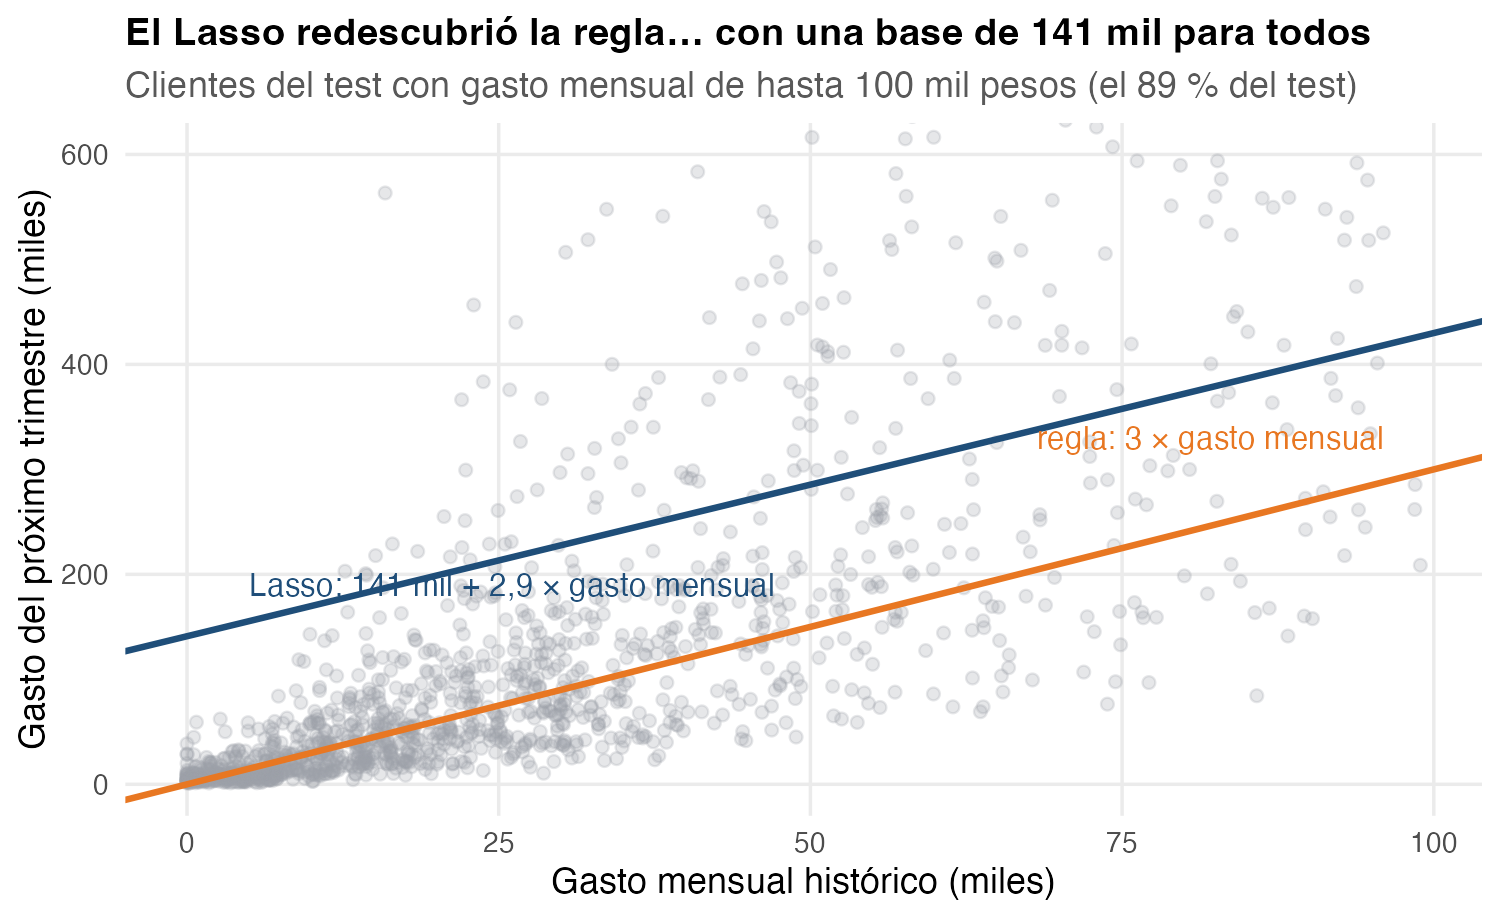
\includegraphics[width=\textwidth]{pic/fig_s12_lasso.png}
\column{0.4\textwidth}
\footnotesize
Minimiza $\text{error}^2 + \lambda \sum |\beta_j|$; $\lambda$ por validación cruzada (\texttt{lambda.1se}).
\begin{itemize} \setlength{\itemsep}{0.06cm}
  \item De \textbf{41 columnas}, sobrevive \textbf{una}: gasto mensual, con coeficiente \textbf{2,888} e intercepto \textbf{141.070}.
  \item Un cliente de 11.020 al mes: predice \textbf{172.898}; gastó \textbf{40.300}.
  \item MAE \textbf{228.481 ± 30.386}; RMSE \textbf{649.069}.
\end{itemize}
\end{columns}
\pause
\vspace{0.1cm}
\begin{alertblock}{Hallazgo 2}
La máquina \textbf{redescubrió la regla de Finanzas}, pero con una base de 141 mil para todos: pierde en MAE (por más que el margen) y gana, apenas, en RMSE. El Lasso gana en la métrica que optimiza.
\end{alertblock}
\end{frame}

\begin{frame}{Paso 3 · ¿Por qué el árbol no se atreve?}
\small
\begin{columns}[T]
\column{0.56\textwidth}
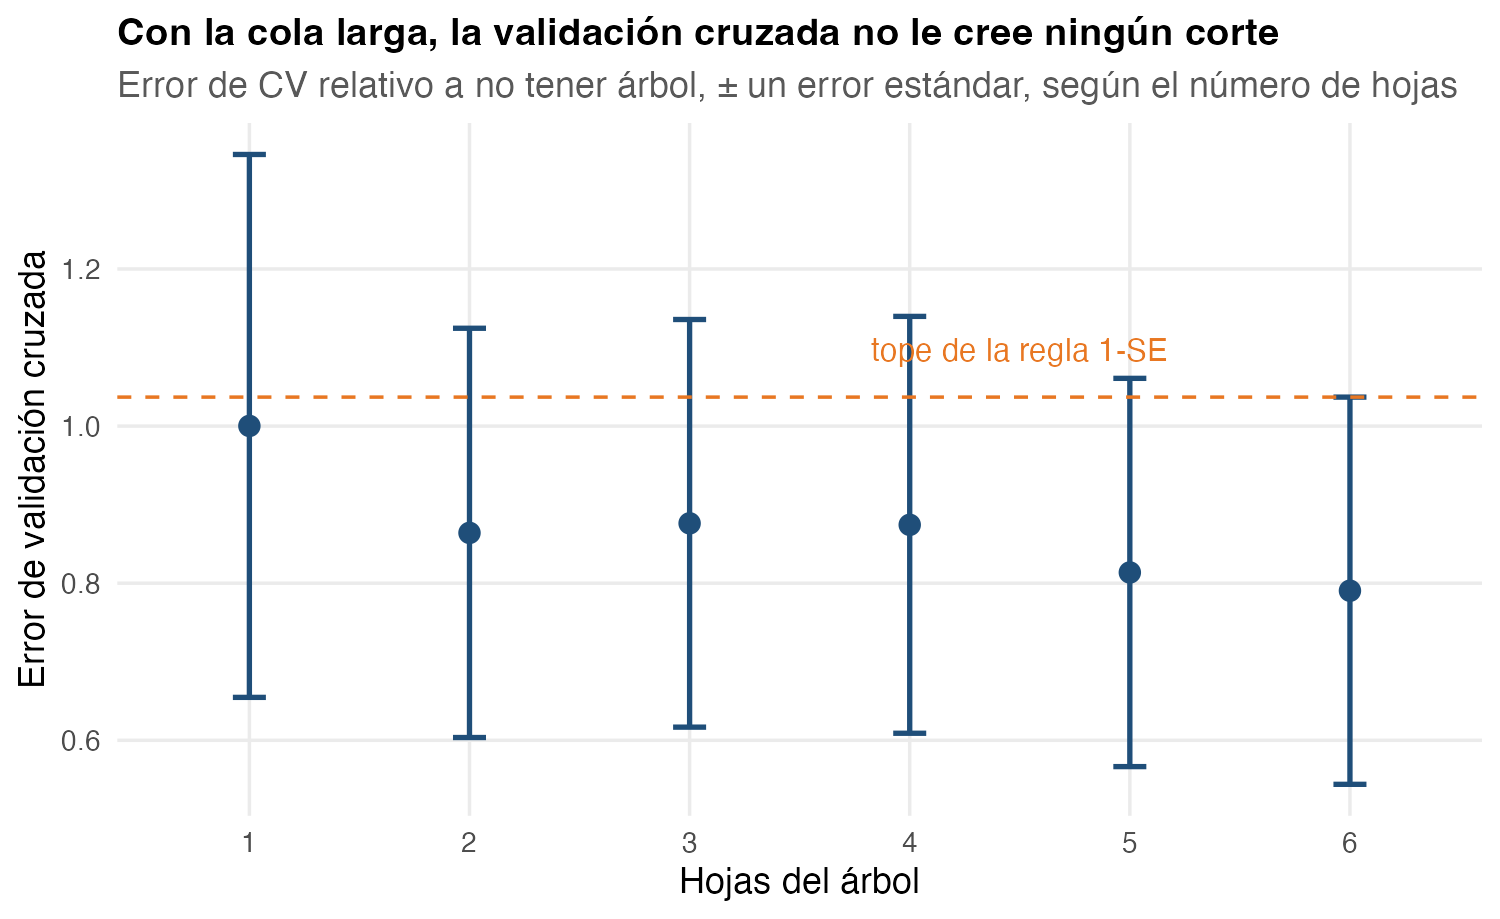
\includegraphics[width=\textwidth]{pic/fig_s12_cv_arbol.png}
\column{0.42\textwidth}
\footnotesize
\begin{itemize} \setlength{\itemsep}{0.06cm}
  \item Sin podar, todas sus preguntas son sobre el gasto mensual; arriba de 883 mil quedan \textbf{22 clientes} con promedio de \textbf{10,8 millones} --- y aun así los parte \textbf{por ciudad}.
  \item En test: RMSE \textbf{869.870}, peor que la media.
  \item Regla 1-SE: tope \textbf{1,037} > 1,000 $\Rightarrow$ \textbf{una sola hoja}: la media.
\end{itemize}
\end{columns}
\pause
\vspace{0.1cm}
\begin{alertblock}{Hallazgo 3}
Con la cola larga, la validación cruzada cambia tanto de pliegue a pliegue que \textbf{no le cree ningún corte}: la inestabilidad del árbol, en su versión extrema --- y la razón de ser del bosque.
\end{alertblock}
\end{frame}

\begin{frame}{Paso 4 · ¿Promediar 500 árboles arregla el árbol?}
\small
\begin{columns}[T]
\column{0.48\textwidth}
\centering
\scriptsize
\begin{tabular}{lr}
\toprule
Bosque (500 árboles) & Test \\
\midrule
MAE & 162.654 ± 29.017 \\
RMSE & 602.535 \\
\bottomrule
\end{tabular}
\column{0.5\textwidth}
\begin{itemize} \setlength{\itemsep}{0.12cm}
  \item El único de hoy que le gana a la regla en las \textbf{dos} métricas.
  \item En la importancia manda, de lejos, el \textbf{gasto mensual}; después, la antigüedad y el monto total.
\end{itemize}
\end{columns}
\pause
\vspace{0.3cm}
\begin{alertblock}{Hallazgo 4}
Promediar sí arregla la inestabilidad: donde un solo árbol no se atrevía, 500 árboles superan a la regla. Y la historia se repite: lo que más dice del gasto futuro es el gasto pasado.
\end{alertblock}
\end{frame}

\begin{frame}{Paso 5 · ¿La ventaja del bosque es real o es ruido?}
\small
\begin{columns}[T]
\column{0.58\textwidth}
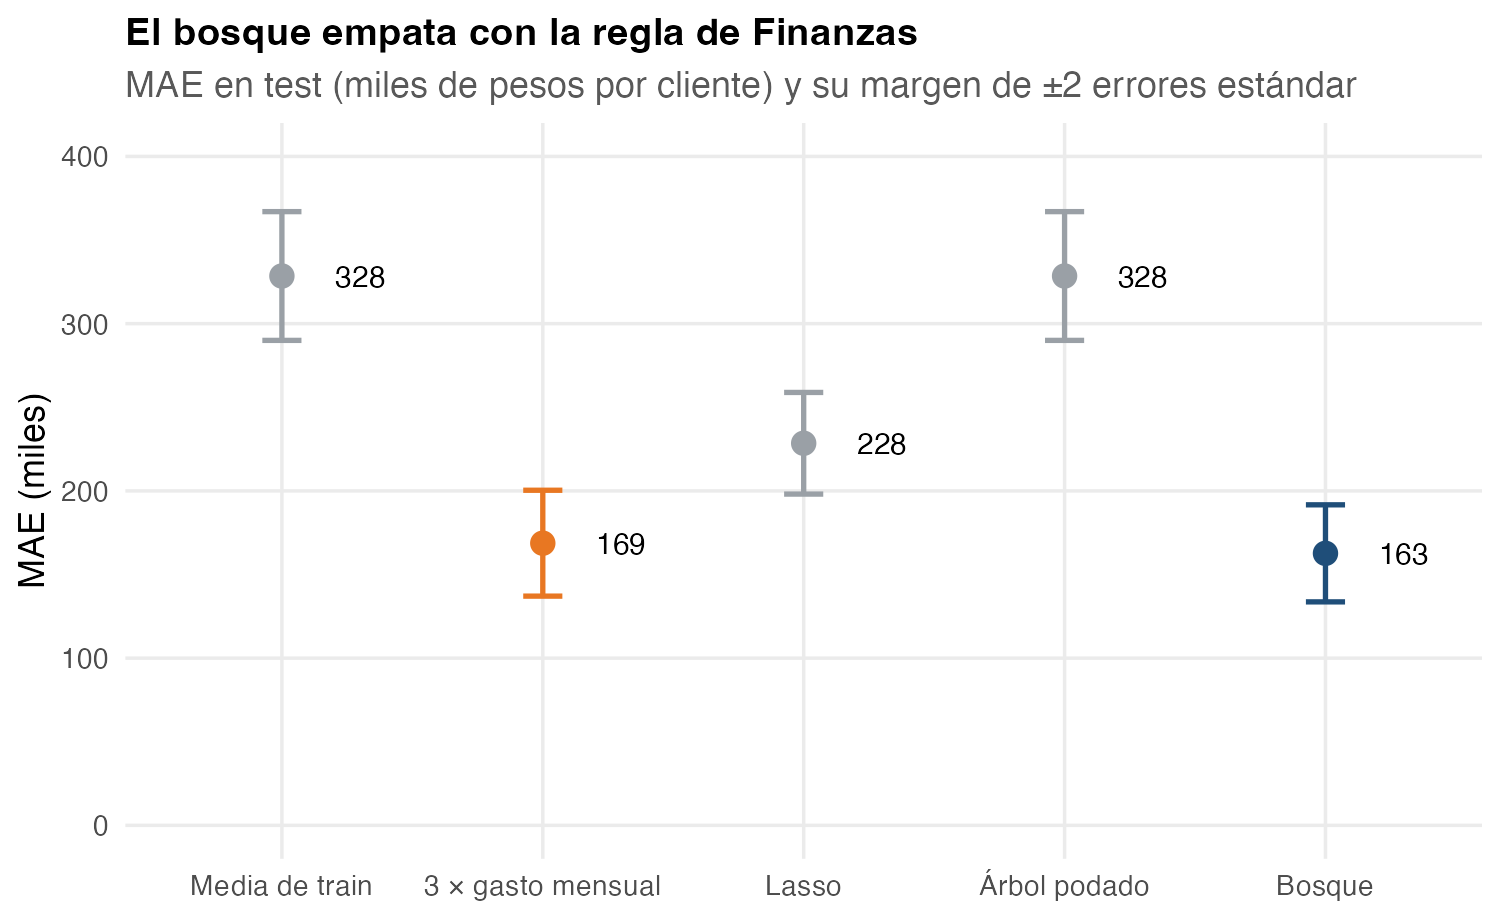
\includegraphics[width=\textwidth]{pic/fig_s12_torneo.png}
\column{0.4\textwidth}
\footnotesize
Cliente a cliente, en el mismo test:
\begin{itemize} \setlength{\itemsep}{0.06cm}
  \item Bosque contra regla: \textbf{6.074 ± 14.429} pesos. El margen alcanza el cero.
  \item Regla contra media: \textbf{159.766 ± 13.679}. Casi doce veces su margen.
\end{itemize}
\end{columns}
\pause
\vspace{0.1cm}
\begin{alertblock}{Hallazgo 5 --- la lección de la semana}
\textbf{Empate técnico} entre el bosque y la regla de Finanzas. La mejora de verdad fue la de la semana 10: casi todo lo que se sabe del gasto futuro ya estaba en el gasto pasado.
\end{alertblock}
\end{frame}

%%=================================================
\section{Dónde falla y a quién llamar}

\begin{frame}[noframenumbering]{Roadmap}
\tableofcontents[currentsection]
\end{frame}

\begin{frame}{Paso 6 · ¿Dónde se equivoca?}
\small
\begin{columns}[T]
\column{0.58\textwidth}
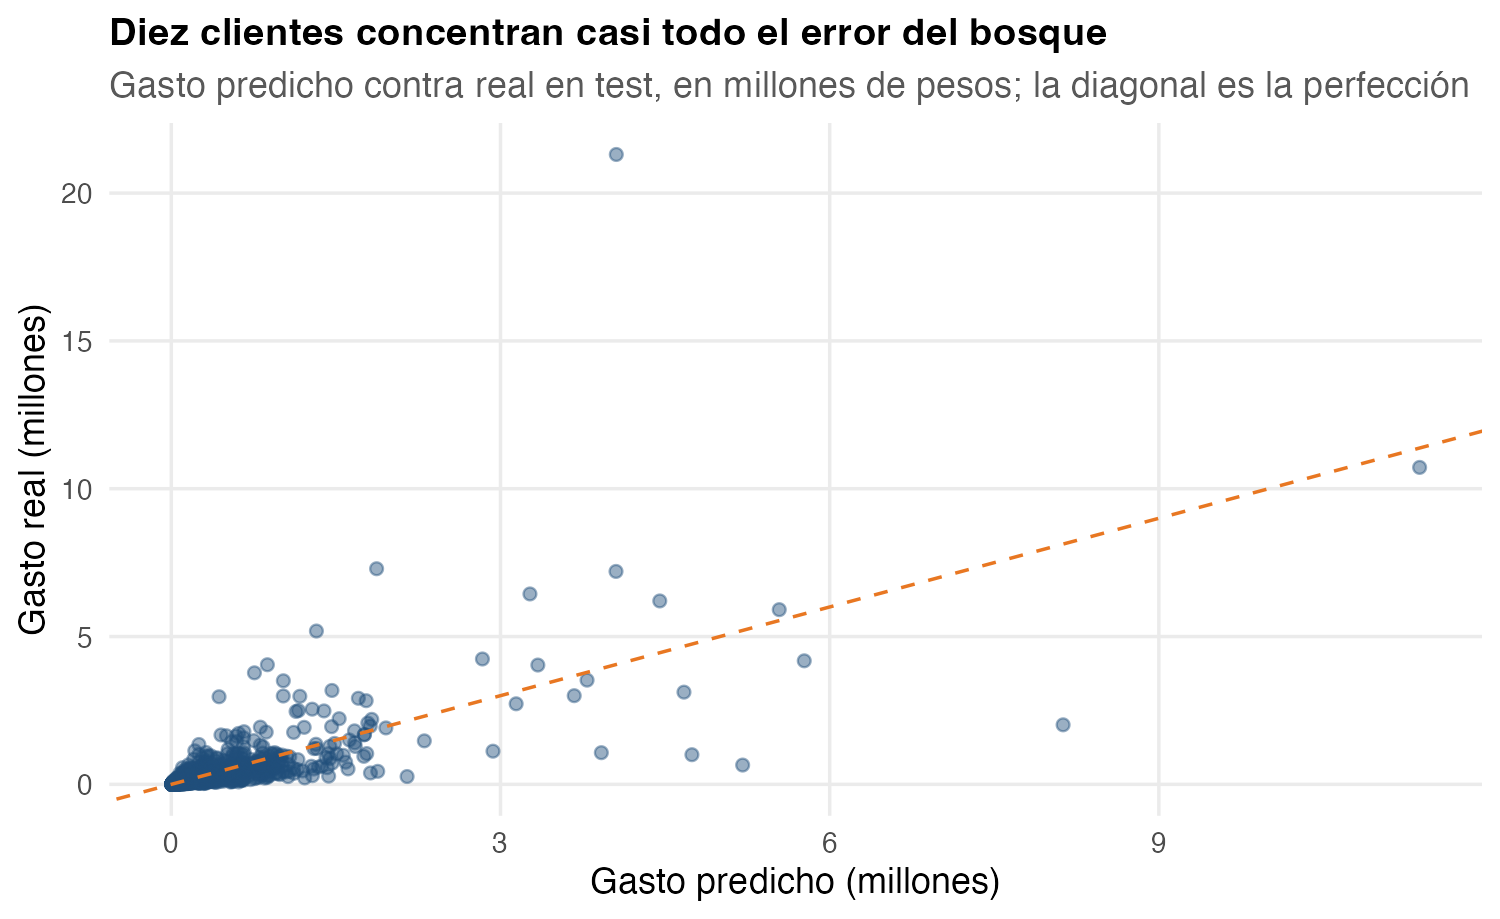
\includegraphics[width=\textwidth]{pic/fig_s12_diagnostico.png}
\column{0.4\textwidth}
\footnotesize
\begin{itemize} \setlength{\itemsep}{0.08cm}
  \item La nube se pega a la diagonal; unos pocos puntos se escapan, por arriba y por abajo.
  \item Un cliente gastó \textbf{21 millones} cuando se esperaban 4.
  \item Los \textbf{10 peores} de 1.600 se llevan el \textbf{78\,\%} del error al cuadrado.
\end{itemize}
\end{columns}
\pause
\vspace{0.1cm}
\begin{alertblock}{Hallazgo 6}
El pronóstico sirve para el 99\,\% de la cartera; los grandes gastadores necesitan \textbf{tratamiento aparte} (un ejecutivo de cuenta, un rango de escenarios). Y eso explica por qué el RMSE queda tan lejos del MAE.
\end{alertblock}
\end{frame}

\begin{frame}{Paso 7 · ¿A quién llama Growth?}
\small
\begin{columns}[T]
\column{0.56\textwidth}
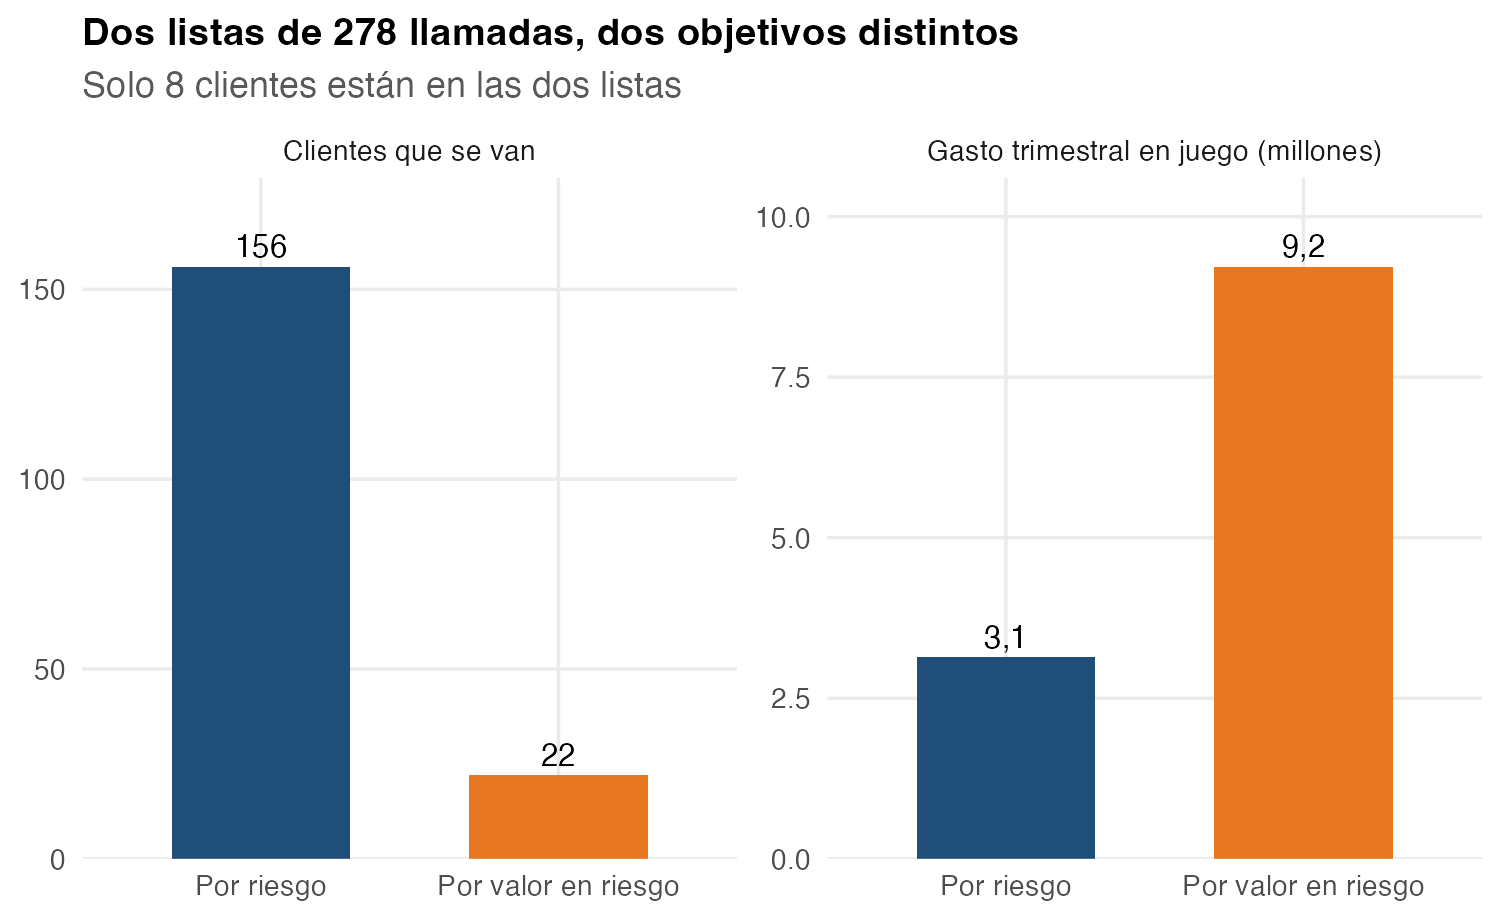
\includegraphics[width=\textwidth]{pic/fig_s12_valor.png}
\column{0.42\textwidth}
\footnotesize
\textbf{Valor en riesgo} = probabilidad de irse (semana 11) × gasto esperado (hoy).
\begin{itemize} \setlength{\itemsep}{0.06cm}
  \item \textbf{Por riesgo}: 156 que se van, gasto esperado mediano de 11.762.
  \item \textbf{Por valor en riesgo}: 22 que se van, mediana de 632.493.
\end{itemize}
\end{columns}
\pause
\vspace{0.1cm}
\begin{alertblock}{La decisión --- no tiene respuesta única}
Si la meta es \textbf{retener clientes}, se llama por riesgo; si es \textbf{retener gasto}, por valor en riesgo: tres veces más plata en juego, aunque la mayoría de las llamadas caiga en clientes que no se iban.
\end{alertblock}
\end{frame}

%%=================================================
\section{Lo que queda}

\begin{frame}[noframenumbering]{Roadmap}
\tableofcontents[currentsection]
\end{frame}

\begin{frame}{La tabla del líder}
\small
\centering
\footnotesize
\textbf{Gasto del próximo trimestre} (pesos por cliente, test de 1.600)
\vspace{0.05cm}

\begin{tabular}{lcr}
\toprule
Regla o modelo & MAE & RMSE \\
\midrule
Media de train & 328.494 ± 38.496 & 836.839 \\
\rowcolor{grisclaro} \textbf{3 × gasto mensual} & 168.728 ± 31.656 & 655.018 \\
Lasso (\texttt{lambda.1se}) & 228.481 ± 30.386 & 649.069 \\
Árbol podado & 328.494 ± 38.496 & 836.839 \\
\rowcolor{grisclaro} \textbf{Bosque} & 162.654 ± 29.017 & 602.535 \\
\bottomrule
\end{tabular}

\raggedright
\small
\pause
\vspace{0.25cm}
\begin{block}{La decisión}
El bosque encabeza la tabla, pero su ventaja sobre la regla de Finanzas cabe en el margen: \textbf{colíderes}. Si hay que explicarle a Finanzas cómo se pronostica, gana la regla de una línea.
\end{block}
\end{frame}

\begin{frame}{Qué produce un torneo de regresión --- y qué no}
\small
\begin{columns}[T]
\column{0.48\textwidth}
\textbf{Produce}
\begin{itemize} \setlength{\itemsep}{0.1cm}
  \item Un pronóstico para cada cliente, con su error típico en pesos.
  \item Un diagnóstico: dónde falla y qué segmento pide otro tratamiento.
  \item El valor en riesgo, junto con la semana 11.
\end{itemize}
\column{0.48\textwidth}
\textbf{No produce}
\begin{itemize} \setlength{\itemsep}{0.1cm}
  \item Causas: el coeficiente del Lasso \emph{se asocia} con el gasto; no dice que subir el gasto de hoy suba el de mañana.
  \item Más señal que la que hay: con estos datos, casi todo estaba en el gasto pasado.
  \item Certeza con los extremos: diez clientes deciden el RMSE.
\end{itemize}
\end{columns}
\end{frame}

\end{document}
